\documentclass{article}
\usepackage[utf8]{inputenc}
\usepackage{amsmath}
\usepackage{amsthm}
\usepackage[left=1in,right=1in,top=0.9in,bottom=0.9in]{geometry}
\usepackage{graphicx}
\usepackage{float}
\usepackage{titling}
\usepackage{algorithm}
\usepackage[noend]{algpseudocode}
\setlength{\droptitle}{-1.5cm}
\setlength\parindent{0pt}

\makeatletter
\def\BState{\State\hskip-\ALG@thistlm}
\makeatother


\title{Homework Report}
\date{Last modified: \today}
\author{Shawn Seymour\\ University of Minnesota Morris}

\newtheorem*{definition}{Definition}
\newtheorem{prop}{Proposition}
\newtheorem*{theorem}{Theorem}

\begin{document}

\maketitle

\section*{Heuristics}
In this report, I will discuss multiple vertex coloring heuristics. I will define them as follows:

\subsection*{Heuristic A}

Heuristic A is the greedy algorithm. The input is a simple graph \(G = (V, E)\).

\begin{algorithm}
\caption{Greedy algorithm}
\begin{algorithmic}[1]
\State Label each vertex in $V$, i.e. $v_1, v_2, \dots, v_n$
\For{each $v \in V$}
\State Assign a color $p_i$ to $v_i$ using the smallest available $p_i$
\EndFor
\end{algorithmic}
\end{algorithm}

\subsection*{Heuristic B}

Heuristic B is the greedy algorithm with degree sequencing. It orders the vertices according to the decreasing value of their degree. This is also known as the Welsh-Powell algorithm, which is defined in \cite{welsh}.

\begin{algorithm}
\caption{Welsh-Powell algorithm}
\begin{algorithmic}[1]
\State Label each vertex in $V$, i.e. $v_1, v_2, \dots, v_n$, such that $d_G(v_1) \geq d_G(v_2) \geq \dots \geq d_G(v_n)$
\ForAll{$v \in V$}
\State Assign a color $p_i$ to $v_i$ using the smallest available $p_i$
\EndFor
\end{algorithmic}
\end{algorithm}

\section*{Findings}

\begin{prop}
Heuristic A and Heuristic B do not always produce an optimal solution, i.e. they do not always produce a minimum coloring of a graph.
\end{prop}

I will show this for \emph{heuristic B}. It is trivial to show the same for \emph{heuristic A} as \emph{heuristic B} includes the same steps as \emph{heuristic A}. I will construct a simple graph, \(G = (V, E)\), such that:

\begin{align}
|V| &\geq 8 \\
\chi(G) &> \chi^{*}(G)
\end{align}

Let \(\chi\) refer to the coloring of \(G\) generated by \emph{heuristic B}. Let \(\chi^{*}\) be the optimal coloring of \(G\).

\subsection*{Example 1}
I constructed a simple graph, \(G = (V, E)\), such that \(\Delta(G) = 3\) and \(\delta(G) = 1\). I've let \(|V| = 8\) for this example.

\begin{figure}[H]
\centering
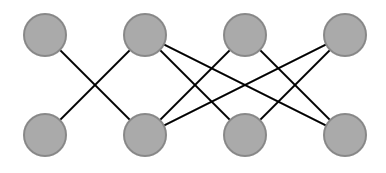
\includegraphics[scale=0.6]{images/graph-1.png}
\caption{Uncolored original graph \(G\)}
\end{figure}

By applying \emph{heuristic B}, we get the following coloring. The numbers indicate the ordering of vertices before applying the heuristic. Any vertex of the same degree got assigned arbitrarily. This results in \(\chi(G) = 3\).

\begin{figure}[H]
\centering
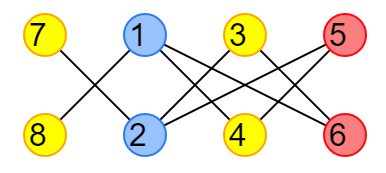
\includegraphics[scale=0.6]{images/graph-2.png}
\caption{Coloring from applying heuristic B}
\end{figure}

\begin{definition}[Bipartite graph]
A bipartite graph is one whose vertex set can be partitioned into two subsets X and Y such that each edge has one end in X and one end in Y
\end{definition}

We can see that this is a bipartite graph, defined above by \cite{bondymurty}. Thus, \(G\) is \emph{2-colorable}. This means \(\chi^{*}(G) = 2\). \(G\) is an example graph that satisfies conditions \((1)\) and \((2)\). The optimal coloring is shown below.

\begin{figure}[H]
\centering
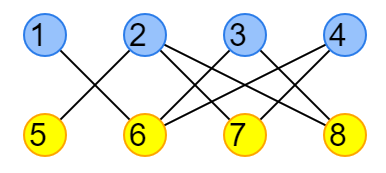
\includegraphics[scale=0.6]{images/graph-3.png}
\caption{Optimal coloring of graph \(G\)}
\end{figure}


\begin{prop}
Heuristic A and heuristic B have an upper bound of \(\Delta + 1\).
\end{prop}

To show this, I will create another example that satisfies conditions \((1)\) and \((2)\) from above. After doing some research into bipartite graphs, I learned that \emph{crown graphs} are excellent at showing how bad greedy heuristics can be, as shown and defined in \cite{kordecki}.

\begin{definition}[Crown Graph]
A crown graph \(CR_n = (V, E)\) is an undirected graph with two sets of vertices where \(V = V_1 \cup V_2\) with an edge from \(v_i \in V_1\) to \(v_{j} \in V_2\) whenever \(i \neq j\). A crown graph can also be viewed as a complete bipartite graph where the edges of a perfect matching have been removed.
\end{definition}

\subsection*{Example 2}

I constructed a simple crown graph, \(H = (V, E)\). I've let \(|V| = 10\) for this example.

\begin{figure}[H]
\centering
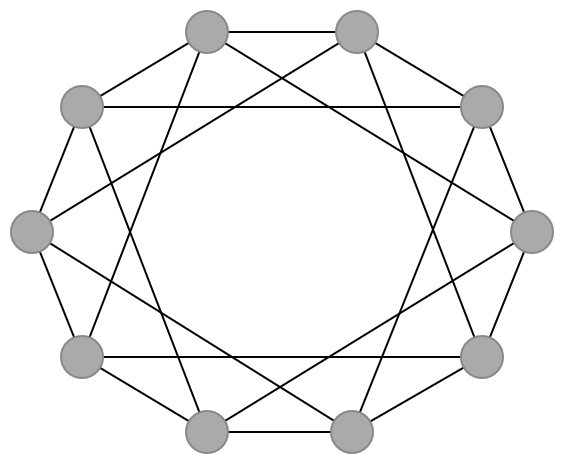
\includegraphics[scale=0.38]{images/graph-4.png}
\caption{Uncolored original graph \(H\)}
\end{figure}

We can see that \(\Delta(G) = 4\). We can also see \(d_G(v) = 4\) for all \(v \in V\). Thus, in both heuristics A and B, the greedy algorithm would pick an order arbitrarily. We can show using this crown graph the worst-case scenario of these heuristics.

\begin{figure}[H]
\centering
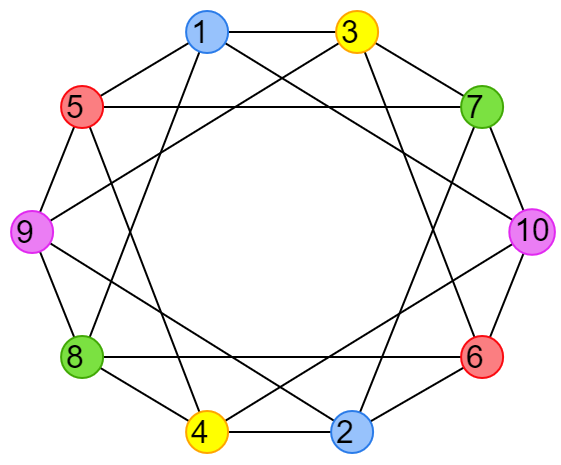
\includegraphics[scale=0.38]{images/graph-5.png}
\caption{Worst-case coloring of \(H\) using either heuristic A or B}
\end{figure}

In Figure 5, using either heuristic with this ordering, we get \(\chi(H) = 5\). This gives us \(\frac{|V|}{2}\) colors. This is the worst-case for a crown graph as shown in \cite{johnson}, but this graph also demonstrates the upper bounds for these heuristics. \newline

\textbf{In General}: Let's take a look at how this looks in general. Let \(P = (V, E)\) be a simple, complete graph. \newline

We can see that \(\chi(H) = \Delta(H) + 1\). This is very easy to see in a \emph{complete} graph, where all vertices are connected to every other vertex. This means all vertices have degree \(|V| - 1\). Thus, every time we color a node, a new color is needed. And since we have \(\Delta(P) = |V| - 1\) and \(|V|\) vertices, we will need \(\Delta(P) + 1\) colors. This is stated in \emph{Brooks' Theorem}.

\newpage

\begin{theorem}[Brooks' Theorem]
For any connected undirected graph \(G\) with maximum degree \(\Delta\), the chromatic number of \(G\) is at most \(\Delta\) unless \(G\) is a complete graph or an odd cycle, in which case the chromatic number is \(\Delta + 1\).
\end{theorem}

The proof of \emph{Brook's Theorem} can be found in \cite{lovasz}. Overall, heuristic A and heuristic B can produce some very undesirable results. In graph \(H\), at the worst case, these heuristics produce \(\chi(H) = 5\) when \(\chi^{*}(H) = 2\) as it is bipartite. This is shown below.

\begin{figure}[H]
\centering
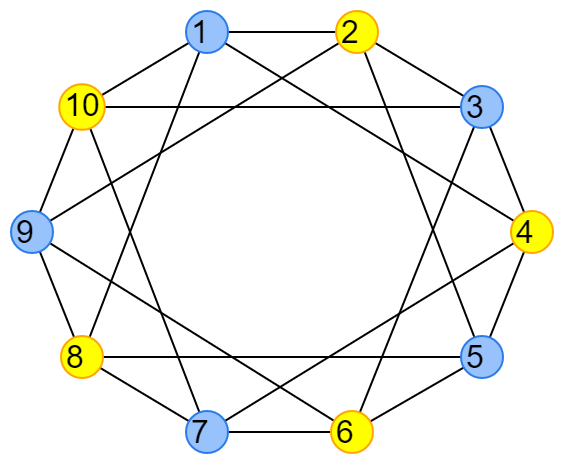
\includegraphics[scale=0.38]{images/graph-6.png}
\caption{Optimal coloring of \(H\)}
\end{figure}



\begin{thebibliography}{9}
\bibitem{bondymurty}
Bondy, J.A. and U.S.R. Murty [1976],
\emph{Graph Theory with Applications},
American Elsevier Publishing, New York, NY.

\bibitem{johnson}
Johnson, D. S. [1974], \emph{Worst-case behavior of graph coloring algorithms}, Proc. 5th Southeastern Conf. on Combinatorics, Graph Theory, and Computing, Utilitas Mathematicae, Winnipeg, pp. 513–527.

\bibitem{kordecki}
Kordecki, W. and A. Łyczkowska-Hanćkowiak [2016], \emph{Greedy online colouring with buffering}, arXiv preprint arXiv:1601.00252.

\bibitem{lovasz}
Lovász, L. [1975], \emph{Three short proofs in graph theory}, Journal of Combinatorial Theory, Series B, 19(3), 269-271.

\bibitem{welsh}
Welsh, D. J. and Powell, M. B. [1967], \emph{An upper bound for the chromatic number of a graph and its application to timetabling problems}, The Computer Journal, 10(1), 85-86.

\end{thebibliography}


\end{document}
